\documentclass[spanish]{textolivre}

% metadata
\journalname{Texto Livre}
\thevolume{17}
%\thenumber{1} % old template
\theyear{2024}
\receiveddate{\DTMdisplaydate{2024}{2}{27}{-1}}
\accepteddate{\DTMdisplaydate{2024}{4}{17}{-1}}
\publisheddate{\DTMdisplaydate{2024}{6}{13}{-1}}
\corrauthor{Manuel Fernando Ramos Nunez}
\articledoi{10.1590/1983-3652.2024.51392}
%\articleid{NNNN} % if the article ID is not the last 5 numbers of its DOI, provide it using \articleid{} commmand 
% list of available sesscions in the journal: articles, dossier, reports, essays, reviews, interviews, editorial
\articlesessionname{articles}
\runningauthor{Sánchez Rivas et al.}
%\editorname{Leonardo Araújo} % old template
\sectioneditorname{Hugo Heredia Ponce}
\layouteditorname{João Mesquita}

\title{Revisión de la producción científica sobre Storytelling mediado por tecnología entre 2019 y 2022 a través de SCOPUS}
\othertitle{Revisão da produção científica sobre Storytelling mediado por tecnologia entre 2019 e 2022 através do SCOPUS}
\othertitle{Review of scientific production concerning Storytelling mediated by technology between 2019 and 2022 through SCOPUS}

\author[1]{Enrique Sánchez Rivas~\orcid{0000-0003-2518-2026}\thanks{Email: \href{mailto:enriquesr@uma.es}{enriquesr@uma.es}}}
\author[1]{Manuel Fernando Ramos Núnez~\orcid{0000-0002-5991-5454}\thanks{Email: \href{mailto:fernandelaware@gmail.com}{fernandelaware@gmail.com}}}
\author[1]{José Sánchez Rodríguez~\orcid{0000-0003-4525-8761}\thanks{Email: \href{mailto:josesanchez@uma.es}{josesanchez@uma.es}}}
\author[1]{María Rubio-Gragera ~\orcid{0000-0002-8311-8498}\thanks{Email: \href{mailto:jmrubiogr@uma.es}{mrubiogr@uma.es}}}

\affil[1]{Universidad de Málaga, Facultad de Ciencias de la Educación, Departamento de Didáctica y Organización Escolar, Málaga, España.}

\addbibresource{article.bib}
\usepackage{csquotes}

\begin{document}
\maketitle
\begin{polyabstract}
\begin{abstract}
El poder de la narración de historias, conocido como “Storytelling”, se ha revelado como una técnica eficaz e indispensable para la transmisión del conocimiento en el ámbito educativo. Este artículo ofrece un estudio de las publicaciones científicas indexadas que respaldan el uso didáctico de las historias mediado por tecnología. El periodo seleccionado abarca desde 2019 hasta 2022. Para realizar la revisión, se aplicó un algoritmo de búsqueda basado en criterios específicos, mediante los que se realizó una revisión de la base de datos SCOPUS. Los datos obtenidos se interpretaron desde una perspectiva cuantitativa, para después aportar un estudio cualitativo mediante el análisis e interpretación de las aportaciones de cada uno de los artículos. Se evidencia un aumento anual y progresivo en la producción científica, con un estancamiento en 2020, y se identifica a los autores, investigaciones e instituciones con mayores aportaciones en el campo objeto de estudio. En cuanto al análisis del contenido, en primer lugar, podemos destacar un creciente interés de la comunidad educativa por la necesidad de construir narrativas que contribuyan a mejorar las metodologías activas en el aula, así como de la integración de estas en entornos tecnológicos. Como fruto de esta tendencia identificamos el auge del uso de términos como “Narración Transmedia”, “Entornos Inteligentes de Aprendizaje” y “Realidad Aumentada”, que están proliferando y abriendo nuevas vías de investigación. Otra de las tendencias destacables puede enmarcarse en el ámbito medioambiental, con numerosos estudios que persiguen reinventar narrativas para concienciar sobre la necesidad de frenar el cambio climático. Por último, detectamos también la utilización de las narrativas para mejorar procesos médicos y terapéuticos, especialmente aplicados a la formación de nuevos profesionales.

\keywords{Ciencias sociales \sep Tecnologías \sep Educación \sep Creatividad \sep Estudio bibliométrico}
\end{abstract}

\begin{portuguese}
\begin{abstract}
O poder da narração de histórias tornou-se uma técnica eficaz e essencial para a transmissão de conhecimentos na Educação. Este artigo apresenta uma revisão de publicações científicas indexadas que apoiam o uso didático de histórias mediadas por tecnologia. A linha do tempo selecionada é de 2019 a 2022. Para esta revisão, foi aplicado um algoritmo de busca baseado em critérios específicos, que apoiou a realização de uma revisão da base de dados SCOPUS. Os dados obtidos foram interpretados a partir de uma perspetiva quantitativa. Em seguida, foi feito um estudo qualitativo através de uma análise e interpretação dos contributos de cada um dos artigos. Evidencia-se um aumento anual e progressivo da produção científica, embora também se observe uma parada em 2020. São também identificados os autores, os trabalhos de investigação e as instituições com maiores contributos nesse domínio. Quanto à análise de conteúdo, em primeiro lugar, podemos destacar um interesse crescente da comunidade educativa na necessidade de construir narrativas que contribuam para melhorar as metodologias ativas na sala de aula, bem como a integração destas em ambientes tecnológicos. Como resultado dessa tendência, identificamos o surgimento do uso de termos como "Narrativa Transmídia", "Ambientes Inteligentes de Aprendizagem" e "Realidade Aumentada", que estão proliferando e abrindo novas vias de pesquisa. Outra tendência destacável pode ser enquadrada no âmbito ambiental, com numerosos estudos que buscam reinventar narrativas para consciencializar sobre a necessidade de combater as mudanças climáticas. Por fim, também detectamos uma ampla utilização das narrativas para melhorar processos médicos e terapêuticos, especialmente aplicados à formação de novos profissionais.

\keywords{Ciências sociais \sep Tecnologias \sep Educação \sep Criatividade \sep Estudo bibliométrico}
\end{abstract}
\end{portuguese}

\begin{english}
\begin{abstract}
The power of storytelling has become an effective and essential technique for knowledge transmission in Education. This article provides a review of indexed scientific publications that support the didactic use of stories mediated by technology. The selected timeline is from 2019 to 2022. For this review, a search algorithm was applied based on specific criteria, that helped to make a review of the SCOPUS database. The obtained data were interpreted from a quantitative perspective. After this, a qualitative study was made by an analysis and interpretation of the contributions of each of the articles. A yearly and progressive increase in scientific production is evidenced, although it is also observed a standstill in 2020. Authors, research works, and institutions with the greatest contributions in this field are also identified. Regarding content analysis, firstly, we can highlight a growing interest from the educational community in the need to construct narratives that contribute to improving active methodologies in the classroom, as well as their integration into technological environments. As a result of this trend, we identify the rise of terms such as "Transmedia Narration," "Intelligent Learning Environments," and "Augmented Reality," which are proliferating and opening new avenues of research. Another noteworthy trend can be framed in the environmental field, with numerous studies seeking to reinvent narratives to raise awareness about the need to curb climate change. Finally, we also detect a significant use of narratives to enhance medical and therapeutic processes, especially applied to the training of new professionals.
    
\keywords{Social sciences \sep Technologies \sep Education \sep Creativity \sep Bibliometric study}
\end{abstract}
\end{english}
\end{polyabstract}

\section{Introducción}\label{sec-Introducción}

La evolución de la inteligencia artificial (IA) ha marcado un hito
significativo en la actualidad sofocada por infodemia e infoxicación.
Esta transformación tecnológica, inicialmente concebida por John
McCarthy en 1956, ha avanzado significativamente, incorporando
aplicaciones de aprendizaje automático y procesamiento del lenguaje
natural (NLP) en herramientas educativas \cite{Sadiku2021}. No obstante, el gran salto se dio con la presentación de
ChatGPT en 2020, y con mejor respuesta a principios del 2023, siendo la
IA Generativa (IAGen) otra forma de entender a la IA; la IAGen crea
contenido original a partir de datos existentes mediante algoritmos y
redes neuronales avanzadas \cite{Feuerriegel2024}.

En el campo de la educación, los modelos de lenguaje grandes (LLM,
\emph{Large Language Model}), como ChatGPT \cite{OpenAI2023}, ha generado
diversos debates públicos y digitales como el de la opinión emitida por
el lingüista {\textcite{Chomsky2023}}, donde califica a ChatGPT como una forma de plagio de alta
tecnología, pudiendo socavar la educación al motivar a los estudiantes
en la búsqueda de atajos para la entrega de trabajos, como los ya
clásicos ensayos o resolución a preguntas cerradas, como en un
cuestionario de reforzamiento, por ejemplo. Ante este tipo de
reflexiones, han surgido otras como la de \textcite{Yell2023}, un
profesor retirado de la Universidad de Wisconsin, argumentan sobre que,
si se utiliza de forma adecuada, ChatGPT puede ser un recurso valioso
para fomentar el aprendizaje basado en la búsqueda e investigación,
permitiendo promover el pensamiento crítico. Aunque es indiscutible que
este tipo de tecnología es capaz de crear contenido nuevo en formato de
texto, imágenes o audio, permitiendo hasta asistir en tareas de
conocimiento y necesidades cotidianas \cite{Feuerriegel2024}.

La aplicación de ChatGPT en la educación se ve reflejada en el análisis
de \textcite{Dimitriadou2023}, quienes abordan la integración de la
IA en las aulas inteligentes y los desafíos éticos asociados, así como
en el estudio de \textcite{Tlili2023} abordando el uso de
\emph{chatbots}, que examinan la aplicación de ChatGPT en la elaboración
de ejercicios en forma de cuestionarios. Estos enfoques resaltan el
equilibrio necesario entre las capacidades de la IA y la intervención
humana para garantizar la relevancia, la exactitud y la equidad en la
educación.

Recientes investigaciones, como las de \textcite{Nasution2023} y \textcite{Ruiz2023},
han explorado el uso de ChatGPT 4.0 en la generación de ítems de examen,
destacando no solo su capacidad para crear preguntas de elección
múltiple relevantes y coherentes, sino también abordando desafíos como
irregularidades y redundancias en interacciones más prolongadas. Estos
estudios subrayan la importancia de la especificidad y sistematización
en los prompts para generar exámenes eficientes y precisos,
capitalizando las fortalezas de la IA para la educación \cite{Nasution2023, Ruiz2023}.

La investigación de \textcite{Nasution2023} se enfocó en la validez y
confiabilidad de las preguntas generadas por IA, un tema que ha
suscitado tanto interés como preocupación en la comunidad educativa. Con
una muestra de 272 estudiantes, Nasution emprendió la tarea de evaluar
una serie de preguntas creadas por ChatGPT, obteniendo resultados que
son tanto prometedores como reveladores. De las 21 preguntas generadas
por la IA, 20 resultaron ser válidas, lo que indica una alta tasa de
éxito. Este hallazgo es significativo, ya que subraya la capacidad de la
IA para producir contenido educativo que no solo es relevante, sino
también de calidad.

No obstante, también hay investigaciones en torno al uso de Machine
Learning (ML) como el de \textcite{Rauber2024} quienes desarrollaron un
modelo automatizado para medir el aprendizaje de conceptos y prácticas
de clasificación de imágenes mediante redes neuronales. Se basó en datos
de 240 estudiantes de secundaria y bachillerato, concluyendo que la
evaluación es confiable y válida. Además, destacaron la efectividad del
modelo resaltando la importancia de incluir ML en la educación escolar y
la capacidad del modelo para asistir en el proceso de evaluación,
facilitando la carga de trabajo de los docentes.

A medida que la tecnología de IA continúa evolucionando, con avances
significativos en las versiones más recientes de ChatGPT, se presenta
una oportunidad única para mejorar y sistematizar el proceso de creación
de exámenes. Las investigaciones de \textcite{Nasution2023,Ruiz2023} se
alinean con esta visión, proponiendo un enfoque metodológico que combina
la exploración y descripción detallada de las capacidades de ChatGPT 4.0
en la generación de ítems de examen, proporcionando así una perspectiva
integral de su aplicabilidad y eficacia en el ámbito educativo. No
obstante, todavía hacen falta estudios que comparen el comportamiento de
la IAGen y si los seres humanos somos capaces de detectar esas
diferencias, o bien, podrían ayudar a reducir la carga de los docentes e
instituciones al momento de crear exámenes de alto impacto; como los del
ingreso a la universidad.

Ante todos estos acontecimientos, y retomando estos modelos de lenguaje
que podrían ayudarnos a evaluar nuestra propia forma de comunicar, el
objetivo principal de esta investigación fue explorar y comparar la
eficacia de la IAGen, representada por ChatGPT 4.0, y los diseñadores
humanos en el desarrollo de ítems para el Examen de Ingreso a la
Educación Superior (ExIES), en el área de Lengua Escrita, a través del
método de juicio de expertos. Lo anterior, con el fin determinar la
calidad, relevancia y alineación de los ítems generados por ambas
fuentes (IA y humanos) con los estándares establecidos para la
evaluación educativa, centrándose en aspectos como claridad,
neutralidad, concisión, alineación curricular y adecuación de formato y
contenido.
\section{Metodologia}\label{sec-metodologia}

Não foi necessária uma análise ética prévia por parte dos conselhos de
projetos adequados para a investigação, uma vez que os participantes não
foram identificados. Por não haver conflito de interesses, a Texto Livre
não terá quaisquer consequências, inclusive assistência integral e
eventual, ressarcimento de qualquer dano resultante a qualquer dos
participantes da pesquisa, conforme a Resolução nº 510, de 7 de abril de
2016, do Conselho Nacional de Saúde do Brasil.

A metodologia é a explicação minuciosa, detalhada, rigorosa e exata de
toda a ação desenvolvida no método de trabalho da pesquisa \cite{lakatos2003}. A pesquisa é um estudo de caso, que teve o aluno como
objeto de estudo. \textcite[p. 32]{yin2005} argumenta que o estudo de caso visa a \enquote{conhecer em profundidade o como e o porquê de uma determinada
	situação que se supõe ser única em muitos aspectos, procurando descobrir
	o que há nela de mais essencial e característico}. O estudo de caso é
caracterizado pelo estudo profundo e exaustivo de um ou poucos objetos,
de maneira a permitir o seu conhecimento amplo e detalhado. O caso
experimental caracteriza-se por determinar um objeto de estudo,
selecionar as variáveis que seriam capazes de influenciá-lo, definir as
formas de controle e de observação dos efeitos que a variável produz no
objeto \cite{gil2002}. A coleta dos dados foi realizada em uma escola
secundária do sul de Moçambique. Fizeram parte da amostra 50 alunos do
ensino secundário, selecionados de forma aleatória, dos quais 25
participaram do estudo das PO e aplicação do Q3DM. Os restantes 25
estiveram envolvidos no estudo das SCs e aplicação do GeoGebra. Em ambos
os estudos, todos os alunos experimentaram as aplicações (Q3DM ou
GeoGebra). A pesquisa apresenta um estudo de caso interpretativo, o qual
desenvolve categorias conceituais indutivamente para examinar os
pressupostos iniciais, as intenções e significados das ações e
expressões dos alunos \cite{amado2017}. A compreensão interpretativa é
sustentada a partir do relato pormenorizado da interação dos sujeitos em
seu meio natural \cite{coulon1995}. A visão interpretativa descreveu as
ações dos alunos em ambiente de sala de aula e os significados das ações
no processo de toda a pesquisa \cite{coutinho2011}.

Foi possível, pois, observar e interpretar tudo o que ocorreu, tornando
viável a análise das relações causa-efeito. Foi possível , também,
qualificar as ações dos alunos em todo o processo de aprendizagem, por
meio das interpretações dos significados de seus comportamentos durante
a mediação da aula e as respostas do questionário de satisfação. Além
disso, os dados foram coletados por meio das técnicas de observação do
participante, com tomada de notas e de registro fotográfico, assim como
dos instrumentos de coleta de dados aplicados, como os questionários de
satisfação.

\subsection{Realização das aulas}\label{sub-sec-Realização das aulas}

As aulas consistiram na apresentação de dois temas, PO e SCs, de forma
separada. Para os alunos da 9ª classe, o tema de pesquisa foi PO, e foi
utilizado o Q3DM. A professora primeiramente apresentou o tema,
explicando o que eram POs, dizendo que eram figuras geométricas sobre um
plano que poderiam ser comparadas à sombra do mesmo objeto no horário em
que o sol estaria no ponto mais alto no dia. Depois, demonstrou as
vistas ortogonais do sólido. (Ver \Cref{fig-03}).

\begin{figure}[htpb]
\centering
\begin{minipage}{.5\textwidth}
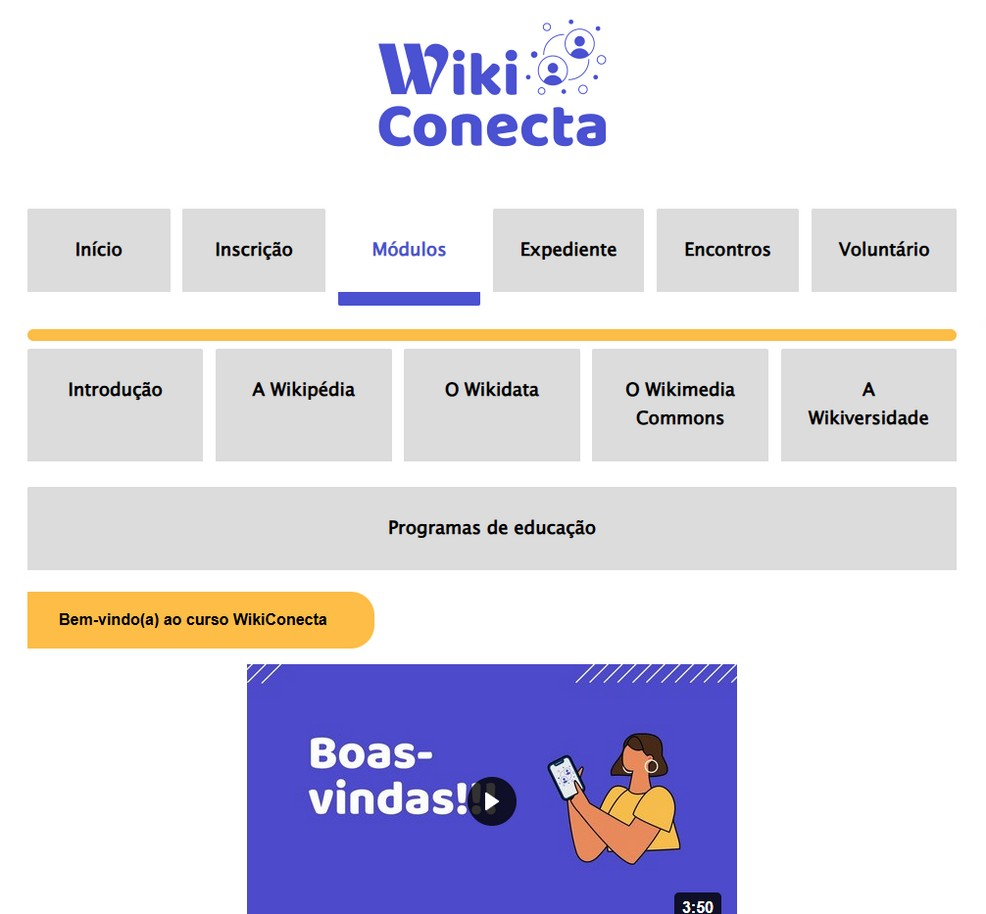
\includegraphics[width=\textwidth]{figures/figure03.jpg}
\caption{Vistas ortogonais e ortográficas: vista frontal; vista superior; e vista lateral esquerda.}
\label{fig-03}
\source{\url{http://turmag1215vialonga.blogspot.com/2014/10/projecoes-ortogonais.html}.}
\end{minipage}
\end{figure}

Posteriormente a professora apresentou a aplicabilidade das POs, dizendo
que eram destinadas à planificação de vários objetos. Com o auxílio das
simulações computacionais, construiu os sólidos geométricos e demonstrou
suas vistas ortogonais, apresentando os procedimentos para a manipulação
do Q3DM. (Ver \Cref{fig-04})

\begin{figure}[htpb]
\centering
\begin{minipage}{.5\textwidth}
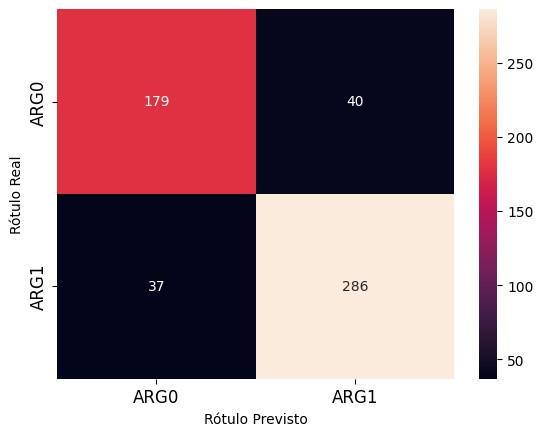
\includegraphics[width=\textwidth]{figures/figure04.jpg}
\caption{Manipulação no Q3DM.}
\label{fig-04}
\source{Elaboração própria.}	
\end{minipage}
\end{figure}


A manipulação no Q3DM é feita por meio de cubos chamados Qubes, que
facilitam a criação e a montagem de objetos em três dimensões,
utilizando elementos digitais que podem ser inseridos, removidos,
deslocados, ampliados, inclinados, moldados geometricamente, girados e
coloridos.

Para os alunos da 12ª classe, o tema de pesquisa foi SCs e foi utilizado
o GeoGebra. A professora iniciou com a apresentação do tema SCs de
cilindro, explicando que a seção cilíndrica é uma figura resultante de
um plano secante no cilindro. A professora acrescentou que existem duas
situações distintas: quando o plano secante é paralelo ao eixo central
do cilindro; e quando o plano secante não é paralelo ao eixo central do
cilindro (ver as figuras \Cref{fig-05} e \Cref{fig-06}).

\begin{figure}[htpb]
\centering
\begin{minipage}{.25\textwidth}
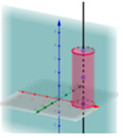
\includegraphics[width=\textwidth]{figures/figure05.jpg}
\caption{Secção paralela ao eixo central do cilindro.}
\label{fig-05}
\source{Elaboração própria.}
\end{minipage}
\end{figure}

\begin{figure}[htpb]
\centering
\begin{minipage}{.5\textwidth}
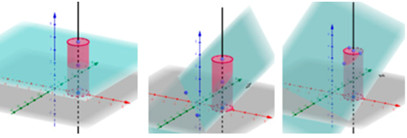
\includegraphics[width=\textwidth]{figures/figure06.jpg}
\caption{Secção não paralela ao eixo central do cilindro.}
\label{fig-06}
\source{Elaboração própria.}
\end{minipage}
\end{figure}

A professora, primeiramente, apresentou os diferentes posicionamentos
dos planos em relação ao eixo central do cilindro. Em seguida, com o
auxílio da tecnologia, apresentou à turma o software de geometria
dinâmica GeoGebra, indicando as funcionalidades de suas ferramentas e
como construir do ponto até o plano secante, com a ajuda dos
procedimentos para a sua manipulação no GeoGebra. Os alunos simularam as
SCs com o plano de nível; eles apresentaram-se atentos e motivados em
aprender a resolver o exercício no GeoGebra, particularmente para os
rapazes, os quais procuravam descobrir como construir diferentes sólidos
geométricos e como simular as VOs (vistas ortogonais).

\subsection{Realização do questionário}\label{sub-sec-Realização do questionário}

O questionário de satisfação aplicado teve como objetivo compreender se
o Q3DM e o GeoGebra facilitaram a aprendizagem das POs e SCs, e se o
\textit{smartphone} foi fácil de manipular. Ambos os questionários foram
preenchidos em 10 minutos. As questões visavam a coletar, nos dois
estudos, várias opiniões, incluindo: (1) se os aplicativos tecnológicos
facilitaram as representações 3D; (2) qual é a opinião deles sobre os
benefícios de usar os aplicativos ou se seria melhor resolver de forma
tradicional; (3) se os aplicativos são fáceis e intuitivos de usar; (4)
quais foram os aspectos positivos e negativos da aula; e, (5) como eles
classificariam a aprendizagem com o auxílio dos aplicativos.

\section{Análisis y resultados}\label{sec-análisisyresultados}

Los resultados de este estudio se representan organizados según los
criterios de análisis establecidos. En primer lugar, se muestran los
números de artículos publicados por periodos temporales, es decir, por
años naturales. En ellos se evidencia un aumento progresivo anual de la
producción, y 2021 como el año con el incremento más pronunciado \Cref{tab-01}.

\begin{table}[htbp]
\centering
\begin{threeparttable}
\caption{Número de artículos por año.}
\label{tab-01}
\begin{tabular}{lll}
\toprule
Año & Artículos & Diferencia\\
\midrule
2019 & 26 & - \\
2020 & 28 & 2 \\
2021 & 40 & 12\\
2022 & 51 & 11\\
\bottomrule
\end{tabular}
\source{Elaboración propia.}
\end{threeparttable}
\end{table}

A partir de 2021 se observa una mayor preocupación por explorar nuevas
fórmulas narrativas. Encontramos una razón para ello en la crisis del
COVID-19. De acuerdo con diversos autores \cite{monroy_retos_2021,torras_virgili_emergency_2021,una_martin_aproximacion_2020,vilhelm_rios_didactica_2022}, consideramos que la
pandemia y la crisis sanitaria reformularon muchos planteamientos
pedagógicos tradicionales, generando la necesidad de experimentar con
modelos más flexibles, personalizados, con tecnologías y metodologías
más innovadoras.

El número de citas de los artículos es muy variable, y no puede
establecerse un patrón de comportamiento, ni correlación entre las
fechas de publicación y el impacto de los artículos. Aunque generalmente
los artículos más antiguos suelen tener mayor número de citas, en el
caso que nos ocupa los dos artículos más destacados fueron publicados en
2021. Entre toda la producción seleccionada, podemos destacar un trabajo
que alcanza más de sesenta citas, y otros siete con cifras superiores o
iguales a veinte \Cref{tab-02}

\begin{table}[htbp]
\centering
\begin{threeparttable}
\caption{Número de citas por año.}
\label{tab-02}
\begin{tabular}{lllll}
\toprule
\multicolumn{1}{c}{Artículo} & \multicolumn{4}{c}{Citas por año} \\
  &2019& 2020& 2021& 2022\\
\midrule
Secundo, Mele, Vecchio, Elia, Margherita, \& Ndou (2021) &-& - &16& 51\\
Agbo, Oyelere, Suhonen, \& Tukianen (2021)& -& - &12 &25\\
Kerr, \& Lawson (2020)& - &6& 16 &11\\
Flórez-Aristizábal \& Fardoun (2019)& 3& 4 &7& 12\\
Naul, \& Liu (2020) &- &1& 9& 15\\
Sarnok, Wannapiroon, \& Nilsook (2019) &1 &4& 8& 10\\
Kaeophanuek, Na-Songkhla, \& Nilsook (2019) & 2 & 4& 8& 7\\
\bottomrule
\end{tabular}
\source{Elaboración propia.}
\end{threeparttable}
\end{table}

Atendiendo al número de citas, debemos destacar tres artículos que están
liderando la tendencia en investigación sobre el \emph{storytelling}
mediado por el uso de tecnología y sus posibilidades pedagógicas. Se
trata de los trabajos de \cite{secundo_threat_2021,agbo_scientific_2021,kerr_augmented_2020}.

El primero de ellos surge en el contexto de crisis del COVID-19, y en él
se abordan los principales retos tecnológicos que la pandemia generó en
el ámbito educativo. Los autores ilustran el rediseño de un programa de
aprendizaje para emprendedores, aprovechando las tecnologías digitales y
a nivel práctico, aportan ideas para remodelar los programas
universitarios tradicionales, preparándolos para abordar emergencias
futuras.

El segundo artículo ofrece una amplia revisión bibliográfica en la que
se examina el panorama de la investigación sobre los Entornos
Inteligentes de Aprendizaje, mediante un análisis bibliométrico. El
resultado de este análisis indica que el primer artículo sobre esta
nueva realidad se publicó en 2002, lo que supuso el inicio en la
exploración de este campo. Los Entornos Inteligentes de Aprendizaje
aluden a entornos físicos enriquecidos con dispositivos digitales,
sensibles al contexto y adaptativos, para promover un aprendizaje más
rápido y eficaz \cite{koper_conditions_2014}. Su análisis temático muestra que la narración digital y sus componentes asociados, como la realidad virtual, el pensamiento crítico y los Juegos Serios, que son juegos creados para proporcionar un contexto de entretenimiento y auto-fortalecimiento con
el que motivar, educar y entrenar a los jugadores  \cite{chipia_lobo_juegos_2011}. Consideramos que se trata de dos líneas de investigación emergentes.

Por último, en el artículo de \cite{kerr_augmented_2020}, se describe el
desarrollo de un prototipo de Realidad Aumentada, creado para formar a
estudiantes en los principios básicos de la arquitectura paisajística.
El enfoque principal de los autores se centra en proponer nuevas
prácticas de narración digital a través de experiencias situadas. De
este trabajo inferimos la necesidad de mejorar los programas de
formación docente para capacitar a los futuros maestros en la
integración de las tecnologías inmersivas, como también indica \cite{figueroa_fusionando_2021}.

El tercer indicador hace referencia a las autorías, y nos permite
destacar a los investigadores que más han aportado en el campo objeto de
estudio. En la siguiente tabla mostramos sus nombres y filiación
institucional, a través de la cual podemos observar una gran
representación de Australia y Malasia país que, junto a Tailandia,
lidera sus investigaciones desde universidades centradas en el
desarrollo tecnológico \Cref{tab-03}.

Este dato se corrobora al confrontarlo con las instituciones destacadas
en la investigación sobre \emph{Storytelling} \Cref{tab-04}.

\begin{table}[htbp]
\centering
\begin{threeparttable}
\caption{Investigadores destacados.}\label{tab-03}
\begin{tabular}{lll}
\toprule
Investigador & Filiación & Artículos\\
\midrule
Nilsook, Prachyanun &King Mongkut´s University of Technology & 3\\
Buendgens-Kosten, Judith & Goethe-Universität Frankfurt am Main & 2\\
Chubko, Nadezhda & Edith Cowan University & 2\\
Cornillie, Frederik & KU Leuven & 2 \\
Girmen, Pınar &  Eskişehir Osmangazi Üniversitesi & 2\\
Kantathanawat, Thiyaporn K. & Mongkut's Institute of Technology Ladkrabang & 2\\
Kantathanawat, Thiyaporn K. & Mongkut\textquotesingle s Institute of Technology Ladkrabang & 2\\
Lummis, Geoff W. & Edith Cowan University& 2\\
Macleroy, Vicky & Goldsmiths, University of London &2\\
McKinnon, David H. & Edith Cowan University & 2\\
Morris, Julia Elizabeth & Edith Cowan University & 2\\
\bottomrule
\end{tabular}
\source{Elaboración propia.}
\end{threeparttable}
\end{table}


Al analizar las filiaciones (\Cref{tab-04}) de los principales autores y producción por
países, encontramos en Europa y América del Norte el mayor volumen de
aportaciones. El continente americano, lidera las investigaciones que
relacionan el \emph{Storytelling} con el ámbito de la medicina y la
salud, aunque también hay una gran representación europea debido a las
aportaciones de Reino Unido. En lo referente al campo de las ciencias
sociales, Europa es quien lidera y marca las tendencias. España, que
ocupa el cuarto puesto de la tabla en número de aportaciones por países
con un total de catorce artículos, destaca por su contribución a los
campos relacionados con la aplicación de la narrativa en entornos
digitales, nuevos soportes, y en el uso de metodologías activas. En este
sentido, podríamos señalar a este país como uno de los líderes en la
investigación sobre innovación y tecnología educativa. Este interés por
el \emph{Storytelling} aplicado a metodologías activas y recursos
digitales, continúa aumentando y ha sido identificado en otros estudios
recientes vinculados a universidades españolas \cite{sanchez-rivas_narrative-based_2022,sanchez_rivas_experiencia_2023}.

\begin{table}[htbp]
\centering
\begin{threeparttable}
\caption{Instituciones destacadas.}
\label{tab-04}
\begin{tabular}{lll}
\toprule
Institución & País & Artículos \\
\midrule
Universiti Kebangsaan & Malasia & 3\\
Goldsmiths, University of London & Reino Unido & 3\\
Universiti Teknologi Malaysia & Malasia & 3\\
King Mongkut\textquotesingle s Institute of Technology Ladkrabang &
Tailandia &3\\
Edge Hill University & Reino Unido & 3\\
National and Kapodistrian University of Athens & Grecia & 3\\
King Mongkut\textquotesingle s University of Technology North Bangkok&
Tailandia &3\\
Universitat Oberta de Catalunya & España & 2\\
Universiti Utara Malaysia & Malasia & 2\\
David Geffen School of Medicine at UCLA & Estados Unidos & 2\\
Universidad de Oviedo& España & 2\\
\bottomrule
\end{tabular}
\source{Elaboración propia.}
\end{threeparttable}
\end{table}

 En lo que respecta a la producción por países, Estados Unidos ocupa la primera posición con veintiuna aportaciones, seguido de Reino Unido y Australia. España ocupa la cuarta posición de la tabla con una aportación de catorce artículos, el mismo número que Australia \Cref{tab-05}.
 
\begin{table}[htbp]
\centering
\begin{threeparttable}
\caption{Producción por países.}
\label{tab-05}
\begin{tabular}{ll}
\toprule
País & Artículos \\
\midrule
Estados Unidos & 21\\
Reino Unido & 19\\
Australia & 14\\
España & 14\\
Grecia & 11\\
Malasia & 10\\
Canadá & 9 \\
Italia & 9\\ 
\bottomrule
\end{tabular}
\source{Elaboración propia.}
\end{threeparttable}
\end{table}

Si atendemos a las líneas de investigación abiertas en relación con el
\emph{Storytelling,} advertimos que su estudio se aborda desde
diferentes disciplinas. Aunque el enfoque de las investigaciones siempre
tiene una perspectiva pedagógica, podemos asegurar que el tratamiento
científico de las mismas se acomete desde una perspectiva
multidisciplinar \Cref{tab-06}.

\begin{table}[htbp]
\centering
\begin{threeparttable}
\caption{Producciones por disciplina científica.}
\label{tab-06}
\begin{tabular}{ll}
\toprule
País & Artículos \\
\midrule
Ciencias Sociales & 107\\
Ciencias Informáticas & 40\\
Artes y Humanidades & 22\\
Ingeniería & 16\\
Medicina & 15\\
Psicología & 15\\
Administración y negocios & 6\\
Ciencias Medioambientales & \\
Ciencia de Materiales & 5\\
Ciencias de la Salud &5\\
\bottomrule
\end{tabular}
\source{Elaboración propia.}
\end{threeparttable}
\end{table}

A la hora de abordar nuestro análisis cualitativo, y dar respuesta a
nuestra primera pregunta de investigación, se realizó un análisis de los
campos de estudio y de los contenidos desde los que se abordaban los
diferentes artículos publicados, es decir, aquellos ámbitos con mayor
interés en el uso de historias como recurso didáctico. Las Ciencias
Sociales, las Ciencias Informáticas y las Artes y Humanidades fueron las
áreas más productivas. Cabe destacar que, si a la medicina le sumamos
las publicaciones de otros campos afines como el de las ciencias de la
salud o el de la psicología, ocuparían el tercer puesto. Esto es debido
a la gran cantidad de estudio de casos que utilizan estas ciencias tanto
para enseñar, como para contrastar información en el desempeño de su
trabajo.

A esta revisión de naturaleza cuantitativa, se añadió otra de tipo
documental, para responder a nuestra segunda pregunta e identificar las
finalidades pedagógicas de las líneas temáticas más investigadas en cada
una de las principales áreas de estudio. Los trabajos analizados podrían
organizarse en tres grandes bloques (\Cref{tab-07}). En primer lugar, aquellos que ponen su foco en el proceso de aprendizaje y utilizan las técnicas vinculadas a las historias para mejorar el proceso didáctico. Dentro de esta vertiente, encontramos una gran tendencia a trasladar los modelos
clásicos de la narración a nuevos medios, soportes y tecnologías. En
segundo lugar, contamos con una gran producción de trabajos enfocados en
la transmisión de valores, concienciación con el medio ambiente, con la
inclusión y la necesidad de eliminar fronteras tecnológicas, sociales, y
étnicas. Por último, encontramos una línea dedicada a utilizar la
narración como cauce terapéutico, destinando sus estrategias y recursos
a mejorar la salud física y mental de las personas.

\begin{table}[htbp]
\centering
\begin{threeparttable}
\caption{Principales finalidades pedagógicas de la narración de historias en los artículos analizados.}
\label{tab-07}
\begin{tabular}{ll}
\toprule
Bloque 1 & Narración de historias como parte del proceso de enseñanza y
aprendizaje.\\
Bloque 2 & Narración de historias como medio de transmisión de valores.\\
Bloque 3 & Narración de historias como cauce terapéutico.\\
\bottomrule
\end{tabular}
\source{Elaboración propia.}
\end{threeparttable}
\end{table}

Al enfrentarnos a nuestra tercera pregunta de investigación, y analizar
los conceptos más mencionados en cada uno de los bloques anteriormente
descritos, en el primero de ellos descubrimos un creciente interés en la
comunidad científica por la necesidad de construir historias que
contribuyan al éxito en la aplicación de las denominadas metodologías
activas en el aula. De esta manera, los términos Aprendizaje Basado en
Proyectos, el Aprendizaje Basado en Resolución de Problemas y el
Aprendizaje Cooperativo, son habituales en los trabajos analizados. Del
mismo modo, se identifica un gran volumen de referencias sobre el uso de
la tecnología y los recursos digitales como herramientas de trabajo. En
este sentido, los términos \enquote{Robot}, \enquote{Narrativa Digital}, \enquote{Mapa Digital}, \enquote{Social Media}, \enquote{Dispositivos móviles}, o \enquote{Realidad Aumentada} son los más mencionados.

Con respecto a los trabajos centrados en la concienciación y transmisión
de valores, el concepto de \enquote{Desarrollo Sostenible} es el más repetido,
y también identificamos un gran interés en lo referido a crear
estrategias dirigidas a frenar el cambio climático, la inclusión de
minorías y la conservación del patrimonio inmaterial de las diferentes
culturas. También detectamos una notable producción enfocada en el
intento de disminuir la brecha digital y la igualdad de oportunidades.

En cuanto al tercer bloque, al analizar el área de la salud y el ámbito
terapéutico, los principales ejes de interés se posicionaron entorno a
conceptos como el acompañamiento a pacientes, el estudio de casos de
éxito en medicina, la atención a niños con trastornos del espectro
autista, las terapias psicológicas con animales y el arte, y el refuerzo
de la autoestima.

Además, cabe destacar que desde todas las áreas específicas de
conocimiento se hallaron dos grandes tendencias. La primera de ellas
referida al concepto \enquote{Narración Transmedia}, entendida como un
proceso en el que los elementos integrales de una historia se dispersan
sistemáticamente a través de múltiples canales de distribución con el
fin de crear una experiencia de entretenimiento unificada y coordinada
\cite{jenkins_transmedia_2010}. El otro núcleo de interés está relacionado con la pandemia del COVID-19, y numerosos artículos inciden en la necesidad de
estructurar la narración para mantener la atención de los estudiantes
durante el proceso de \enquote{e-Learning} o \enquote{Aprendizaje a distancia}, así como de la importancia de emplear la tecnología para conseguirlo. Por último, cabe destacar otros dos campos que están presentes en un gran número de estudios y generando tendencia, que son los \enquote{Entornos Inteligentes de Aprendizaje} y la \enquote{Realidad Aumentada}.

Desde el punto de vista metodológico, encontramos una mayoría de
estudios mixtos, que combinan técnicas cuantitativas y cualitativas,
entre las que destacan los estudios etnográficos. Con respecto a las
investigaciones que derivan de las ramas del área de la salud,
identificamos una gran producción en forma de estudios de casos.

\section{Discusión y conclusiones}\label{sec-discusiónyconclusiones}

Partiendo de los resultados obtenidos, consideramos que se refuerza un
planteamiento, ya apuntado por otros autores \cite{alfian_role_2021,sidorenko-bautista_use_2020}, que
sostiene que las narrativas deben cambiar para adaptarse a los nuevos
medios, y que los medios están cambiando continuamente para adaptarse a
las narrativas. En este sentido, se observa un gran interés de la
comunidad científica por adaptar las técnicas clásicas de la narración a
los nuevos medios, soportes, tecnologías y entornos, para logar conectar
con sus audiencias. La necesidad de vehicular contenidos a través de
estructuras narrativas creíbles resulta esencial ya que, de acuerdo con
\cite{vergara2020herramientas}, podemos decir que si algo nos
caracteriza desde el punto de vista cultural es que somos depredadores
de buenas historias.

Como podemos observar, el interés por el \emph{Storytelling} ha superado
la barrera de las Ciencias Sociales, posicionándose como método de
transmisión de conocimiento en diversas disciplinas. El
\emph{Storytelling} es una herramienta poderosa que ha sido utilizada
durante siglos en una variedad de ámbitos, desde la literatura hasta la
publicidad, desde la política hasta la psicología. Su capacidad para
inspirar, educar y entretener va mucho más allá de las ciencias sociales
\cite{haven_story_2007}.

Los hallazgos que hemos realizado nos permiten concluir que la narrativa
sigue siendo fundamental para la articulación de contenidos y el proceso
de enseñanza y aprendizaje. La comunidad científica muestra un gran
interés por adaptar la narrativas y técnicas del \emph{Storytelling} a
los nuevos escenarios educativos, metodologías y herramientas
tecnológicas. La continua exploración de las posibilidades de estas
técnicas está despertando el interés de diferentes disciplinas que
persiguen beneficiarse del carácter pedagógico de las historias.

Podemos establecer otra línea de conclusiones en relación con las
temáticas que se abordan en las historias. Hemos detectado un gran
interés de la comunidad científica por construir narrativas eficaces que
puedan ayudar a comprender las claves del cambio climático. En este
sentido, resulta interesante la vía abierta por diversos trabajos \cite{arnoud_climate_2018,bloomfield_climate_2021,de_meyer_transforming_2021,moezzi_using_2017} que recomiendan trasladar, utilizando
técnicas de comunicación efectiva, estas narrativas climáticas a todas
las esferas de la sociedad, y no solo al ámbito educativo.

Desde la perspectiva didáctica, se hace evidente el interés por crear
propuestas metodológicas específicas que permitan aprovechar todo el
potencial del \emph{Storytelling} en el aula. Los métodos activos son,
en todos los casos, las opciones preferidas. Entendemos que se trata de
una relación lógica, ya que el Storytelling guarda una relación de
coherencia con los rasgos propios del aprendizaje activo (implicación
emocional, cooperación, creatividad, búsqueda del conocimiento, etc.).
Hemos encontrado diferentes estrategias metodológicas para utilizar las
historias como recurso didáctico. Muchas se integran en el método
didáctico Aprendizaje Basado en Historias.

Otros de los fenómenos a los que la comunidad científica debe prestar
atención en el futuro es al de los \emph{Entornos Inteligentes de
Aprendizaje} y a \emph{la Narración transmedia}. De todas estas nuevas
vías, surgen fortalezas como el potencial pedagógico de las narrativas
aplicadas al pensamiento reflexivo o a los nuevos medios digitales \cite{kim_digital_2021,yasar__2022} y otros debates éticos, como la
moralidad de utilizar técnicas de manipulación, como podría considerarse
el \emph{Storytelling} dentro del contexto de las redes sociales tras
demostrarse los efectos negativos que estas producen en la salud mental
\cite{sheldon_dark_2019}.

En cuanto al uso de la tecnología que todas estas metodologías
combinadas con narrativas propician, se imponen con claridad
instrumentos como los dispositivos móviles y la realidad aumentada. En
este sentido, numerosos autores \cite{aurelia_survey_nodate,dunleavy_augmented_2014,nam_designing_2015,nobrega_mobile_2017} apuntan al potencial de la combinación de ambas tecnologías como un buen modelo de enseñanza debido a que cualquier lugar u objeto del mundo real puede integrarse en una historia, estimulando la imaginación del participante. Aunque también señalan que existen algunas barreras que impiden a los usuarios participar activamente en este tipo de actividades, como la
necesidad de disminuir la brecha digital y el elevado coste de los
dispositivos y la tecnología.

Al contrastar nuestra revisión con otras similares, podemos comprobar
que las conclusiones confluyen en varios aspectos. El primero de ellos
sería en la positiva percepción sobre la aplicación de la narración
digital de historias por parte de los estudiantes. Esta idea ha sido
destacada en otras revisiones que también señalan el efecto novedad como
posible artífice de esta aceptación. Se propone continuar investigando
para ver cómo se desarrolla esta relación en el futuro. El segundo
aspecto a tener en cuenta sería la necesidad de formar a los docentes en
el uso de los entornos digitales y la creación, ya que la narración de
historias continúa capturando la atención de audiencias, convirtiéndose
en un aliado indispensable de cualquier proceso didáctico y formativo,
por lo que necesitamos formar a nuestros docentes \cite{chikasanda_enhancing_2013,lawless_professional_2007}.

En relación con futuras líneas de investigación, cabe apuntar que el
importante índice de experimentación didáctica que hemos encontrado,
unido a la necesidad de una constante adaptación de las narrativas a los
nuevos entornos inteligentes y digitalizados, derivarán en nuevas formas
de enseñar y aprender en el futuro, a las que la comunidad científica
deberá prestar atención para evaluar su potencial y medir su eficacia.


\printbibliography\label{sec-bib}
%conceptualization,datacuration,formalanalysis,funding,investigation,methodology,projadm,resources,software,supervision,validation,visualization,writing,review
\begin{contributors}[sec-contributors]
\authorcontribution{Enrique Sánchez Rivas}[conceptualization,methodology,resources,writing]
\authorcontribution{Manuel Fernando Ramos Núnez}[conceptualization,datacuration,investigation,validation,writing]
\authorcontribution{José Sánchez Rodríguez}[formalanalysis,review,supervision]
\authorcontribution{María Rubio-Gragera}[formalanalysis,review,supervision]
\end{contributors}
\end{document}
